\section{$CO_2$ Modelling}
\subsection{Simple emission model}
\label{Modelling}
A simple model for estimating the emissions from single trips has been developed. The trips are divided into sections by the transportation mode detection algorithm. For each transportation mode a emission factor is calculated and multiplied with the length of the section. The total emission for a trip is calculated by accumulating the emissions from the sections. The emission factors for cars, trucks, busses and trains are derived from the reporting of the national emission inventories to UNFCC under the Kyoto Protocol. 

\subsection{IPCC methodology}
The scientific panel guiding the political decisions made in UNFCC is called IPCC (Intergovernmental Panel for Climate Change). The IPCC has made a number of reports on how to calculate emissions of climate forcing gasses and pollutants. The gasses that IPCC are describing methods for are divided into four groups: 

Group 1 are pollutants where a detailed methodology for estimating the emission from activity data, such as driving conditions, and engine conditions.
\begin{table}[htbp]
  \centering
  \begin{tabular}{@{} | c|c |@{}}
    %\toprule
    %Specie & abbreviation \\ 
    %\midrule
\hline
    Carbon monoxide & CO\\ 
Nitrogen oxides & (NOx: NO and NO2)\\
Volatile organic compounds &(VOCs)\\
Methane &(CH4)\\
Non-methane VOCs &(NMVOCs)\\
Nitrous oxide &(N2O)\\
Ammonia &(NH3)\\
Particulate matter &(PM)\\
\hline
  %  \bottomrule
  \end{tabular}
  \caption{Group 1 species}
  \label{tab:group1}
\end{table}


Group 2 are pollutants which can be estimated from fuel consumption, when there is a direct connection between the burning of fuel and the emission. In this group the pollutants are: 	
\begin{table}[htbp]
  \centering
\begin{tabular}{@{} | c|c |@{}}
\hline
Carbon dioxide & (CO2) \\
Sulphur dioxide & (SO2) \\
Lead & (Pb)\\
Arsenic & (As)\\ 
Cadmium & (Cd)\\ 
Chromium & (Cr) \\
Copper & (Cu)\\
Mercury & (Hg) \\
Nickel & (Ni) \\
Selenium & (Se)\\ 
Zinc & (Zn)\\
\hline
\end{tabular}
  \caption{Group 2 species}
  \label{tab:group2}
\end{table}
The data for the Group 2 pollutants are regarded as precise as the data for the Group 1 pollutants even if the methodology differs.
\begin{table}[htbp]
  \centering
\begin{tabular}{@{} | c|c |@{}}
\hline
Polycyclic aromatic hydrocarbons & (PAHs) \\
Persistent organic pollutants & (POPs)\\
Polychlorinated dibenzo dioxins & (PCCDs)\\
Polychlorinated dibenzo furans &  (PCDFs)\\
\hline
\end{tabular}
  \caption{Group 3 species}
  \label{tab:group3}
\end{table}
Group 3 and Group for pollutants are organic compounds, where no detailed methodology exist for estimating the emission, so simple method is used to calculate the emission.

The fourth group of pollutants are species, where the emission is calculated as a fraction of the Non Methane Volatile Organic Compound (NMVOC).
\begin{table}[htbp]
  \centering
\begin{tabular}{@{} | c|c |@{}}
\hline
Alkanes & (CnH2n+2)\\
Alkenes &(CnH2n)\\
Alkynes & (CnH2n-2)\\
Aldehydes & (CnH2nO)\\
Ketones & (CnH2nO)\\
Cycloalkanes & (CnH2n)\\
Aromatic compounds& -\\
\hline
\end{tabular}
  \caption{Group 4 species}
  \label{tab:group4}
\end{table}
  
When considering Climate forcing gases the most important gasses are in Group 1 and 2, thus this is what the focus has been on in this phd study.

The way emission inventories are created are described in the the Guidelines from IPCC . In the guidelines three different methods ere described, each method more accurate than the previous. 

\subsubsection{IPCC Tier 1 model} \alnote{ Size of data (small)}

The Tier 1 method are based on numbers for national sales of hydrocarbons (Gasoline, Diesel, Natural gas etc.). These numbers are readily available for most countries and are converted into emission inventories by multiplying emissions factors (grams of the specie pr kilogram of fuel) for each type of fuel. The Tier 1 method is the simplest, but also most crude way of estimating the national emissions.

Formulas

\subsubsection{IPCC Tier 2 model} \alnote{ Size of data (large)}
In the Tier 2 method the emission inventories are estimated by estimating the traffic volumes for different categories of vehicles, and multiplying emission factors (gram pr kilometre) for each category. The vehicles are divided into 6 main categories: Passenger Car, Light Duty vehicles, Heavy Duty vehicles, Buses, Mopeds and Motorcycles. For each of the main categories, a subdivision is made, to accommodate for different emission characteristics stemming from pollution regulation, fuel type and engine size. For instance, in Europe, passenger gasoline cars are subdivided into 13 different types, according to the legislation governing allowed emissions. These regulations has been changed and tightened 13 times since the first emission control legislation was ratified in the early nineties. For each vehicle category and vehicle type and legislation class, activity data has to be obtained. The activity data consist of the number of vehicles, and the number of kilometres they drive pr year, for each class. The IPCC has generated tables of emission factors (as g/km) for each class of vehicles. By multiplying these emission factors with the estimated kilometres and number of vehicles in the class, the total emission of a pollutant can be estimated for the vehicle class. The total annual emission from transport can then be calculated as the sum of all the vehicle classes.

Formulas



\subsubsection{IPCC Tier 3 model} 
The Tier 3 method takes the Tier 2 methods and improve on the estimated emission, by also consider the velocity distribution of the travelled distances, and by considering the effects of cold-starts on the total emissions.

There are two ways proposed to calculate the effects of speed on exhaust emissions. Either by dividing the travelled distance into road types with different speed characteristics, i.e. urban, rural and highway. In this case the total emission for a vehicle class will be calculated as the sum of the product of travelled distance on a road type and the emission factor for that road type and vehicle type.

The other method uses a measured speed to emission curve and a speed distribution function to estimate the emission. The emission is calculated as the integral of the speed distribution multiplied by the emission function.

\alnote{MORE formulas}
\begin{equation}
e_{i,k,r} = \int{e(V)*f_{k,r}(V)dv}
\end{equation}

($i$ is the the pollutant for which the emission is calculated).

The data needed to use the Tier 3 method is quite extensive. For each of the 13 vehicle classes (divided by fuel type, vehicle size) activity data for milage for urban, rural and highway travel, hot start/cold start, as well as data for the number of vehicles in each emission regulation is needed. Fortunately the program COPERT 4 contains the emission factors, and country specific activity data can be downloaded to use for evaluating national inventories.


\subsection{Modelling emissions from electric vehicles}
The emissions for electric cars are calculated from near real time emission data from Energinet.dk, under the assumption that electric cars will be charged with electricity from the public grid. There is for now no way to detect if the charging of electric vehicles are not done through the public electric grid.
\subsection {Implementation}
The emission factors for combustion engines, as used in the national emission inventories, are based on measured emissions from standardised test runs, and are used for a bottom up estimate of the total national emissions, by estimating the number of kilometres the total national fleet have driven. This estimate is compared to an estimated emission calculated from the amount of gasoline and diesel sold nationally, and the difference between these two estimates leads to a correction factor for the total national emission.

When using smartphones as mobile sensing devices, a number of different sensors can be used. In the following the builtin accelerometer and the global positioning sensor are considered. The accelerometer sensor, delivers a timestamped accelerometer measurement, consisting of a reading of the 3 axis accelerometer. The accelerometer is a very low power device and can thus be sampled quite frequently ( around 200 Hz ).

The GPS measurements consists of longitude, latitude, altitude, speed, bearing, number of satellites visible, accuracy and a timestamp of the measurement. The GPS sensor contains a radio receiver, and complex logic to decode the radio signal and calculate the data, thus it uses more electric power. To reduce the power drain on the smartphone battery, the GPS can be turned off between readings of the position. 

When calculating the distance travelled between two GPS measurements a Haversine function is used. This function takes the curvature of the earth into account, and therefore gives a more precise value for the distance. The resolution of the test data, does not warrant the use of the Haversine approach, but was chosen in anticipation on more crudely sampled GPS data, due to power conservation considerations.



\begin{figure}[!ht]
\begin{center}
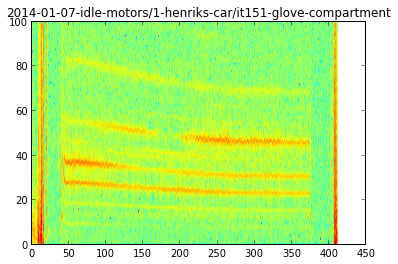
\includegraphics{idle_henrik.png}
\caption{{\bf figure showing rotational speed of an cold engine. As the engine heats up the the engine speed lowers. The yellow colour indicates a larger power.}}
\label{idle_henrik}
\end{center}
\end{figure}



The emission factors are estimated for 3 different driving patterns: Urban, with many stops and low speed. Road driving, with few stops and moderate speeds, and lastly highway, with no stops and high speed. These three modes of road traffic can be distinguished by analysing GPS.  
\begin{figure}[!ht]
\begin{center}
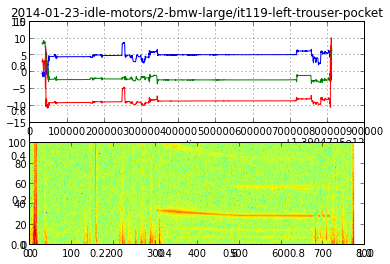
\includegraphics{idle_BMW.png}
\caption{{\bf default}}
\label{idle_bmw}
\end{center}
\end{figure}

To create a more accurate estimate of the emission for a single trip by car, a more complex model is proposed. From the sensed data it is possible to get information on the speed of the car at various points of the trip, and the number of stops and starts. This information can be used to further segment the trips into idle, accelerating, cruising and braking; each of these segments would have a different emission profile. 

The data sensed from the smartphone can also be used to determine if the engine in the car is cold, if for instance it is the start of the trip. When the engine is cold the combustion is less effective and thus more emissions of Carbon Monoxide and Volatile Organic Compounds will be higher and the emission inventory should reflect that. The determination of the impact of cold starts, demands quite complex models, taking into account the outside temperature, models for engine warm up. 
\begin{figure}[htbp]
\begin{center}
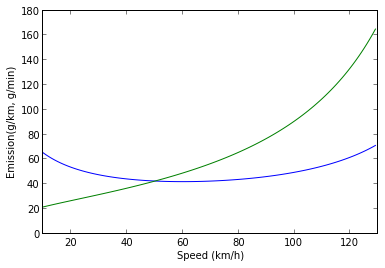
\includegraphics{emission_vs_speed.png}
\caption{{\bf default}}
\label{emission_vs_speed}
\end{center}
\end{figure}


\subsubsection{Determine engine revolutions}
By analysing the frequency spectrum of the accelerometer data, information on the engine revolutions can be retrieved. By employing spectrograms (shows the time evolution of spectral features)  changes in engine speed can be visualised. An example is the the idle speed of a cold motor, where the ECU (Electronic Control Unit) of the vehicle, measures the temperature of the motor and as long as the motor is too cold, sets the idle speed at a higher value. The lowering of the idle speed as the engine grows warmer, is clearly visible in the spectrogram.
The spectrogram is calculated by calculating the size of the accelerometer vector, i.e.:

\begin{center}
$a = \sqrt{x^2+y^2+z^2}$
\end{center}

By calculating the size of the accelerometer vector we do not need to know the exact orientation of the smartphone, and since the gravity can be consider constant the gravity will be present as a signal with frequency equal to zero, which can easily be removed.
The spectrogram shows the time evolution of the frequency spectrum of a signal, so the y-axis shows the frequencies, and the x-axis shows the time. The size of individual frequencies is shown by using different colours. The usefulness of the spectrogram is to show signals with few  frequencies that change slowly, and not to ascertain the exact sir of individual frequencies. The spectrogram can therefore be said to be a qualitative display technique.

During driving, the vibrations from of the moving car, that is the vibrations of from the tires moving over the road and vibrations from the transmission system, drowns the signal of the engine rotational speed.

Another effect that contributes to the loss of a clear signal for the rotational speed of the engine is due to the low sampling frequency of the accelerometer. The sampling frequency of the accelerometer i approximately 200 Hz. This means that the data from the accelerometer only can represent signals with frequency below 100 Hz, due to the Nyquist criteria. This maximum frequency of 100 Hz corresponds to a engine speed of 6000 rpm. Thus the sampling frequency only allows for accurately representation of frequencies below 6000 rpm, and if higher vibrational frequencies exists these frequencies will be folded back into the spectrum from 0 to 6000 rpm, a process called aliasing. Since combustion engines often employ more than one cylinder, and since the process of combustion takes place as a violent process in the cylinder, it is reasonable to expect harmonics of the engine speed to be created. When the engine is in idle mode a rotation of 900 - 1000 rpm is normal and the sampling of the accelerometer will allow the correctly represent up to the 6th harmonic, but when the vehicle is driving engine rotation speed between  
2000 - 3000 would be appropriate, thus only allow to represent third or only second harmonics. Any higher order harmonics will be aliased back into the spectrum and contribute to the noisy picture. 

As a result of vibrational noise from the moving vehicle and aliasing of engine vibration (and aliasing of the vibrational noise for that matter) the signal from the engine rotation is lost in the noise. In signal analysis, the way to prevent aliasing is to apply a low pass filter to remove or dampen frequencies above half the Nyquist frequency. But in our application it is not possible to ensure that the smartphone containing the accelerometer is adequately shielded from high frequency vibrations.

\subsubsection{Determine acceleration and turning}
I order to distinguish between the the four modes of driving (idling,accelerating,cruising, decelerating), which have different emission characteristics, we can use the accelerometer data to determine the the acceleration patterns in the horizontal plane.
The data from the accelerometer is 3 values for each measurement, which are the 3 axis from the accelerometer. The direction of movement of the phone can be determined by analysing these 3 signals. First the direction of gravity is determined. Since it is possible for the phone to be moved freely in all directions and/or flipped with the movement of the person wearing the phone, the gravity detection needs to be dynamic. When the direction of gravity has been determined, it is possible to detect acceleration in the horizontal plane. This allows us to consider distinguishing turning from linear acceleration.

\subsubsection{Combine turning information with GPS }

By combining the turning information, with GPS localisation and map data, the accuracy of the positioning of the car can be improved. Improving the positioning accuracy is important for improving the accuracy of the calculation of trip length and segment of trips length.


The more accurate trip emission estimate would be of interest for instance green accounting purposes.

To validate and compare the models the exact emissions can be measure by inserting a sensor into the exhaust pipe of the vehicle under test. By doing test runs in different kinds of traffic, and with different vehicles the results of the sensor can be compared with the results of the models.